\newpage
\setlength{\parskip}{0.25em}
\renewcommand*{\thefootnote}{\fnsymbol{footnote}}
\setcounter{footnote}{0}
%\makecvtitle
\newcommand*{\cventrynocomma}[7][.25em]{%
	\cvitem[#1]{#2}{%
		{\bfseries#3}%
		\ifthenelse{\equal{#4}{}}{}{ {#4}}%
		\ifthenelse{\equal{#5}{}}{}{ \newline\small #5 \normalfont}%
		\ifthenelse{\equal{#6}{}}{}{ #6}%
		\strut%
		\ifx&#7&%
		\else{\newline{}\begin{minipage}[t]{\linewidth}\small#7\end{minipage}}\fi}}



% ###Design A
%\begin{textblock*}{21cm}(0cm,0cm)	
%	
\includegraphics[scale=1]{./PageDesign/title-eps-converted-d.pdf}
%\end{textblock*}
%\begin{textblock*}{21cm}(2cm,3.4cm)	
%	\Large \textbf{Entwicklung, Simulation}\\[0.8em]
%%	\large{\textbf{Key Skills}}: Stochastic Modelling, Computational Mechanics \normalsize	
%\normalsize
%	\faXing~ \href{https://www.xing.com/profile/Weiran_Zhang4/cv}{Xing} ~ \faLinkedinSquare~ \href{https://www.linkedin.com/in/weiran-zh/}{Linkedin} ~
%	\faCodeFork~ \href{https://github.com/joywezen?tab=repositories}{GitHub}\\
%	% \faGlobe~\href{http://www.weiran.de}{weiran.de}\\		 
%	\faEdit\hspace{0.45em}\href{mailto:weiran-zhang@outlook.com}{weiran-zhang@outlook.com} \\
%	 \faPhoneSquare~ +49~(0)xxxxxx\\	 
%	 %\faMapMarker~~ Braunschweig~~ 
%	 \faWordpress~ \href{http://www.weiran.de}{weiran.de}
%\end{textblock*}

%###Design B



\begin{textblock*}{21cm}(0cm,0cm)	
	
\includegraphics[scale=1]{./PageDesign/title-eps-converted-d.pdf}
\end{textblock*}

\begin{textblock*}{21cm}(2cm,1.7cm)	
	\Huge \textcolor{white}{Weiran Zhang~|}  \Large \textcolor{white}{Entwicklung, Simulation}
\end{textblock*}
\begin{textblock*}{21cm}(2cm,3.2cm)	
%	\Large \textbf{Entwicklung, Simulation}\\[0.8em]
%	\large{\textbf{Key Skills}}: Stochastic Modelling, Computational Mechanics \normalsize	
\normalsize

	\faXing~\href{https://www.xing.com/profile/Weiran_Zhang4/cv}{Xing}\hspace{1em}\faLinkedinSquare~\href{https://www.linkedin.com/in/weiran-zh/}{Linkedin}\hspace{1em}\faCodeFork~\href{https://github.com/joywezen?tab=repositories}{GitHub}\hspace{1em}\faWordpress~ \href{http://www.weiran.de}{weiran.de}\\
	% \faGlobe~\href{http://www.weiran.de}{weiran.de}\\		 
	\faEdit\hspace{0.45em}\href{mailto:weiran-zhang@outlook.com}{weiran-zhang@outlook.com}\hspace{1em}\faPhoneSquare~ +49~(0)xxxxx
	 %\faMapMarker~~ Braunschweig~~ 

	
\end{textblock*}
\begin{textblock*}{21cm}(2cm,4.5cm)	
Soft-Skills:~ $\bullet$ Service- und Teamorientiert ~ $\bullet$ Lernbereit\\
	Fachkompetenzen:~ $\bullet$ Stochastik ~ $\bullet$ Wissenschaftliches Rechnen
\end{textblock*}


\begin{textblock*}{21cm}(15cm,1.2cm)	

	\begin{tikzpicture}[overlay]
	\node[opacity=1] at (2.2,-2.7)%%2.5,-2.3
	{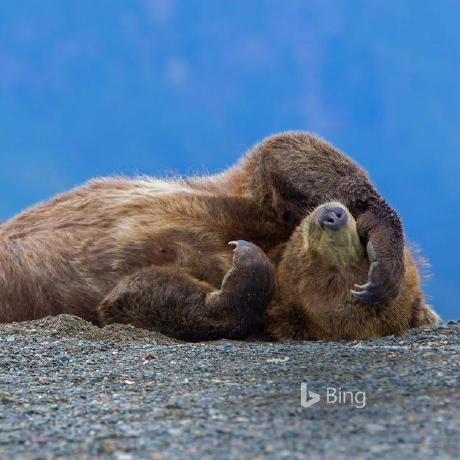
\includegraphics[scale=0.0574]{./PageDesign/YourPic.jpg}}; % add YourPic.jpg in the upper directory "PageDesign"
	\end{tikzpicture}
\end{textblock*}
\begin{textblock*}{21cm}(16.3cm,25cm)	
	
\end{textblock*}
\vspace*{10.5em} 		
	\section{Arbeitserfahrungen}
	
\cventrynocomma{}{*Wissenschaftlicher Mitarbeiter}{\hfill \normalfont \underline{11/2016 - 10/2019}}{Institut für Baumechanik und Numerische Mechanik, Uni Hannover, Deutschland}{}{
	\textbf{$\bullet$\hspace{0.63em}Schädigung- und Werkstoffmechanik, Stochastische Zuverlässigkeitsanalyse}
	%, \textbf{Numerische mechanics}	
	\begin{itemize}%
		%\item[\textit{Tasks}:] %\begin{itemize} DFG founded international training project
		\item Stochastische Materialmodellierung durch Zufallsprozess.
		%\item Zuverlässigkeitsschätzung von Werkstoffstrukturen mittels Monte-Carlo-Simulation.  %stochastische Prozess  
		\item Vorhersage der Sicherheit und Lebensdauer von Bauteilen. 
		%
		%	(z.B. 3Mon. gedauert Experiment wird innerhalb 10Min. simuliert.)  
			%\item Monte-Carlo simulation of stochastic process for structure reliability assessment.
			%\item High performance  non-linear FE analysis for high-cycle fatigue (one million cycles in minutes).
			%\item Large scale data visualisation.
%			\item  with life-cycle prediction.
%		\end{itemize} 
 	\end{itemize}
 	\textbf{$\bullet$\hspace{0.63em}Koordination wissenschaftlicher Veranstaltungen, Betreuung von Studierenden}
 	\begin{itemize}
 		\item Als Koordinator zuständig für Institut-Seminar (2017) und Winter-School (2018). 
 		\item Betreute zwei Bachelorarbeiten und eine Masterarbeit.
 	\end{itemize}
}
 
  \cventrynocomma{}{Gastforscher}{\hfill\normalfont {\underline{01/2019 - 07/2019}}}{Laboratoire de Mécanique et Technologie, Universit\'e Paris-Saclay, Frankreich}{}{
 	\textbf{$\bullet$\hspace{0.63em}Algorithmenentwicklung, Daten-Analyse} 
 	\begin{itemize}
 			\item Finite-Elemente-Berechnung der Ermüdungsschädigung. 
 		%\item  Optische Messung von mechanischer Verformung und Rissentwicklung im Betonträger.
 		%\item Parallelisierte Berechnung von lokalen FE-Moduls, Extrapolation von Zeitreihendaten. % Distributed computing, parallelisation of local FE module,  model extrapolation. 
 		\item Visualisierung, Statistik und Regressionsanalyse von Mess- und Berechnungsdaten.
 \end{itemize}}
 
\cventrynocomma{}{*Studentische Hilfskraft}{\hfill\normalfont \underline{03/2015 - 03/2016}}{Institut für  Wissenschaftliches Rechnen, TU Braunschweig, Deutschland}{}{
	\textit{\textbf{$\bullet$}}\hspace{0.63em}\textbf{Sensor-Fusion, Parameter-Identifikation} 
	\begin{itemize}%  
		\item Daten-Assimilation mittels 4D-Variation und Ensemble-Kalman-Filter (EnKF).
		\item Identifikation der Materialparameter und geometrischer Unsicherheit mit Sensordaten.
		%Referenzlösung erstellt mittels Open-Source-FEA-Software FEAP (entwickelt von UC Berkeley).%Geometrische Parameter-Identifikation aus einer Stahlplatte unter Spannung und Kompressionstest. Das Ziel war um die Position und Größe einer kreisförmigen Aufnahme in einer Stahlplatte zu identifizieren. Der Stand und Messdaten wurden auf der Open-Source Finite-Elemente Software FEAP (UC Berkeley) simuliert, doch der Posterior wurde durch EnKF identifiziert.  %For the simulation is used the ensemble Kalman filter and FE software FEAP (UC Berkeley).
\end{itemize}}

\cventrynocomma{}{Prozess Ingenieur~}{\small -Yutong Bus, Zhengzhou, China \normalsize \hfill\normalfont \underline{06/2013 - 09/2013}}{}{}{\begin{itemize}%
		\item 
		Statistische Qualitätskontrolle  der Elektrophorese-Behandlungsprozessen.
\end{itemize}}
\cventrynocomma{}{Qualitätsingenieur-Oberfläche~}{\small -\textit{Praktikum}, Xi'an Aero-Engine, Xi'an, China\hfill\normalsize \underline{06/2012 - 07/2012}}{}{}{\begin{itemize}%
		\item Oberflächeninspektion und Qualitätskontrolle der
		Triebwerksblätter mittels CMM.
\end{itemize}}
\cventrynocomma{}{Computertechniker~}{\small -\textit{Teilzeit}, Hasee Computer, Zhengzhou, China \normalsize \hfill  \underline{01/2011 - 06/2013}}{}{}{
	\begin{itemize}%
		\item Os- und Hardwarewartung, Aufbauen von Sicherheitssystemen.
	\end{itemize}
}
%\cventry{\normalfont \underline{07/2009 - 06/2013}}{IT-Administrator}{Teilzeit}{Yuke Technology}{Zhengzhou, China}{
%	\begin{itemize}%
%		\item Systemwartung Linux-Server.
%\end{itemize}}
\section{Ausbildungen}
\cventry{\normalfont \underline{11/2016 - 11/2020}}{\textbf{Promotion in Numerischer Mechanik}}{Note: {sehr gut}}{\newline  Leibniz Universität Hannover, Deutschland}{}{
\begin{itemize}%	
	\item[$\bullet$] \textit{Dissertation: {Stochastishe Modellierung und Numerische Simulation von Ermüdungsschädigung.}}
	\item Finite-Elemente-Analyse (FEA), Paralleles Rechnen.
	\item Werkstoffmechanik, stochastischer Prozess.
	%	\item Im Vergleich mit klassischen Monte-Carlo, bezüglich die Berechnungskosten.
\end{itemize}
}
\cventry{\normalfont \underline{10/2013 - 05/2016}}{M.Sc. \textbf{Computational Sciences in Engineering (CSE)}}{Note: 2,1}{}{\newline Technische Universität Braunschweig, Deutschland}{
	\begin{itemize}
		\item Bayessche Statistik, Festkörper- und Strömungsmechanik.
		\item Numerische Verfahren für Differenzialgleichungen, Linear- und Nichtlineare Systemen. 
		%	\item Masterarbeit \textit{Note:\textbf{1,3}}, Projektarbeit \textit{Note:\textbf{1,0}}.
		%	\hspace{-1em}*\hspace{1em}  \item gute Kenntnisse in Datenanalyse und Verarbeitung.
\end{itemize}} 
%\begin{textblock*}{2cm}(2cm,22.5cm)
%	*  
%\end{textblock*}
\footnotetext{* Arbeitszeugnisse wurden beigefügt.} 
%\footnotetext{* Dissertation wurde am 16.06.2020 abgegeben.}
%\hspace*{-0.4cm}
% arguments 3 to 6 can be left empty
\cventry{\normalfont \underline{09/2009 - 06/2013}}{B.Ing. \textbf{Qualität- und Zuverlässigkeit-Ingenieurwissen}}{GPA: 83/100}{}{\newline Zhengzhou University of Aeronautics, China}{\begin{itemize}
		\item Total-Quality-Management (TQM), Qualitätsoptimierung.
		%	\item  Total-Quality-Management (TQM).
		\item Toolkit zur Zuverlässigkeitsanalyse.  
		%		\item , ERP.
\end{itemize}}
%\newpage
%\vspace{-2em}
\section{Studien- und Abschlussarbeiten}
%\hspace*{-0.4cm}
\cventry{\normalfont \underline{10/2015 - 04/2016}}{*Masterarbeit}{Note: {1,3}}{}{TU Braunschweig}{
	\textit{\textbf{$\bullet$}}\hspace{0.63em}\textbf{Unsicherheitsquantifizierung} des Schadens im Betonträger durch Multi-Level-Monte-Carlo-Verfahren
	\begin{itemize}%
		\item Schädigungsmodellierung von Stahlbeton.
		\item Modellierung unsicherer Materialeigenschaften mittels Zufallsfelder.
	%	\item Im Vergleich mit klassischen Monte-Carlo, bezüglich die Berechnungskosten.
\end{itemize}} 
\footnotetext{* Demonstriert im beigefügten Portfolio (in englischer Sprache).}
\cventry{\normalfont \underline{11/2014 - 05/2015}}{*Projektarbeit} {Note: {1,0}}{}{TU Braunschweig}{
	\textit{\textbf{$\bullet$}}\hspace{0.63em}\textbf{Datenassimilation} durch Ensemble Kalman Filter und 4D Variationsmethode
	\begin{itemize}%
		\item Vergleich der Effizienz und Genauigkeit beider Methoden.
		\item  Lösen mehrdimensionales chaotisches System durch 4-stufigen Runge-Kutta Verfahren.
\end{itemize}}
\cventry{\normalfont \underline{12/2012 - 05/2013}}{Bachelorarbeit}{Note: {sehr gut}}{Zhengzhou University of Aeronautics}{}{\textit{\textbf{$\bullet$}}\hspace{0.63em}\textbf{Qualitätsoptimierung} von Bankdienstleistungen aus technischer Perspekt.
	\begin{itemize}%
		\item Hauptkomponentenanalyse des multivariaten Bewertungsmodells der Servicequalität.
		\item Topologiebasierte Service-Netzwerk-Optimierung.
		\item  Ergonomische Verbesserung der Zugänglichkeit von Geldautomaten.
\end{itemize}}


	\section{Weitere Fähigkeiten und Interessen}
\cvitem{Software}{Matlab, Abaqus (mit Python-script), SPSS.}{}{}
\cvitem{Coding}{C++ (QT, Python-test), Python (Pandas, Scipy, TensorFlow).}
%							\cvitem{\hspace{-1cm}Programming}{Matlab, Python}{}{}
\cvitem{Sprachen}{Deutsch (fließend), English (fließend), Mandarin (Muttersprache).}{}{}
%	\cvitem{Sprachen}{English (Arbeitssprache), Chinese (Muttersprache), French \& Portugiese (Grundkenntnisse) }{}{}
%		\cvitem{}{\hspace{5.2em}EU/China Führerschein vorhanden (ohne Verkehrsverstöße seit 5 Jahren)}{}{}
%\cvitem{Licenses}{EU and chinese driving license}{}{}
\cvitem{Hobbys}{Sportfishing, Saxophon, Fotografieren.}{}{}
%\hspace{-2em}*\hspace{2em} 
%, EU and Chinese driving license
%\begin{textblock*}{2cm}(2cm,18.1cm)
%*  
%\end{textblock*}
% arguments 3 to 6 can be left empty

\section{Vorträge bei internationalen akademischen Veranstaltungen}
%\cventry{\normalfont (Dez. 2017)}{Senlis, Frankreich}{}{7th International Conference Fatigue Design}{}{}
\cventry{\normalfont \underline{05/2018}}{Poitier, Frankreich}{}{12th International Fatigue Congress}{}{\textit{Vortrag: On the time discritisation effect of stochastic damage evolution.}}
\cventry{\normalfont \underline{06/2019}}{Crete, Griechenland}{}{3rd International Conference on Uncertainty Quantification \newline in Computational Sciences and Engineering}{}{\textit{Vortrag: Stochastic modelling of fatigue process.}}
\cventry{\normalfont \underline{09/2019}}{Barcelona, Spanien}{}{15th International Conference on Computational Plasticity}{}{\textit{Vortrag: Modelling approach and efficient numerical scheme for stochastic fatigue process.}}
\section{Veröffentlichung}
Stochastic Material Modeling for Fatigue Damage Analysis. \textit{W.Zhang, A.Fau, U.Nackenhorst, R.Desmorat}\newline In: Virtual Design and Validation. Springer, Cham, 2020. S. 329-347. [In englischer Sprache] 
							
								\section{Auszeichnungen}
								\cventry{\normalfont \underline{11/2013}}{CSE "Junior"-Stipendium}{}{}{}{Technische Universität Braunschweig. Braunschweig, Deutschland}
								\cventry{\normalfont \underline{06/2013}}{		"Ausgezeichneter Absolvent"}{}{}{}{Zhengzhou University of Aeronautics. Zhengzhou, China}
								\cventry{\normalfont \underline{10/2012}}{Stipendium Jahr 2012}{}{}{}{Zhengzhou University of Aeronautics. Zhengzhou, China}
								\cventry{\normalfont \underline{09/2011}}{1. Platz bei studentischem Karriereplanwettbewerb}{}{}{}{Zhengzhou University of Aeronautics. Zhengzhou, China}
								\cventry{\normalfont \underline{06/2011}}{2. Platz bei studentischem Musikwettbewerb der Provinz Henan}{}{}{}{Musician Association of Henan Province, Zhengzhou, China}
								\clearpage
